\documentclass[a4paper,12pt]{report}
\renewcommand{\chaptername}{Question}
\renewcommand{\thechapter}{Q.\arabic{chapter}}
\usepackage[margin=0.5in]{geometry}
\usepackage{hyperref}
\usepackage{graphicx}
\usepackage{amsmath}
\usepackage{amsfonts}
\usepackage{amssymb}
%\usepackage{lipsum}
\usepackage{pdfpages}
%\usepackage[pdfpagelabels,hyperindex,hyperfigures]{hyperref}
% Title Page
\title{\textbf{EEE 526 Exam Report}}
\author{Komolafe Elisha Ayobami\\ EEG/2015/061}
\date{November 16, 2021}

\begin{document}
{\Huge \maketitle}
\pdfbookmark[0]{Honor Code}{Honor Code}
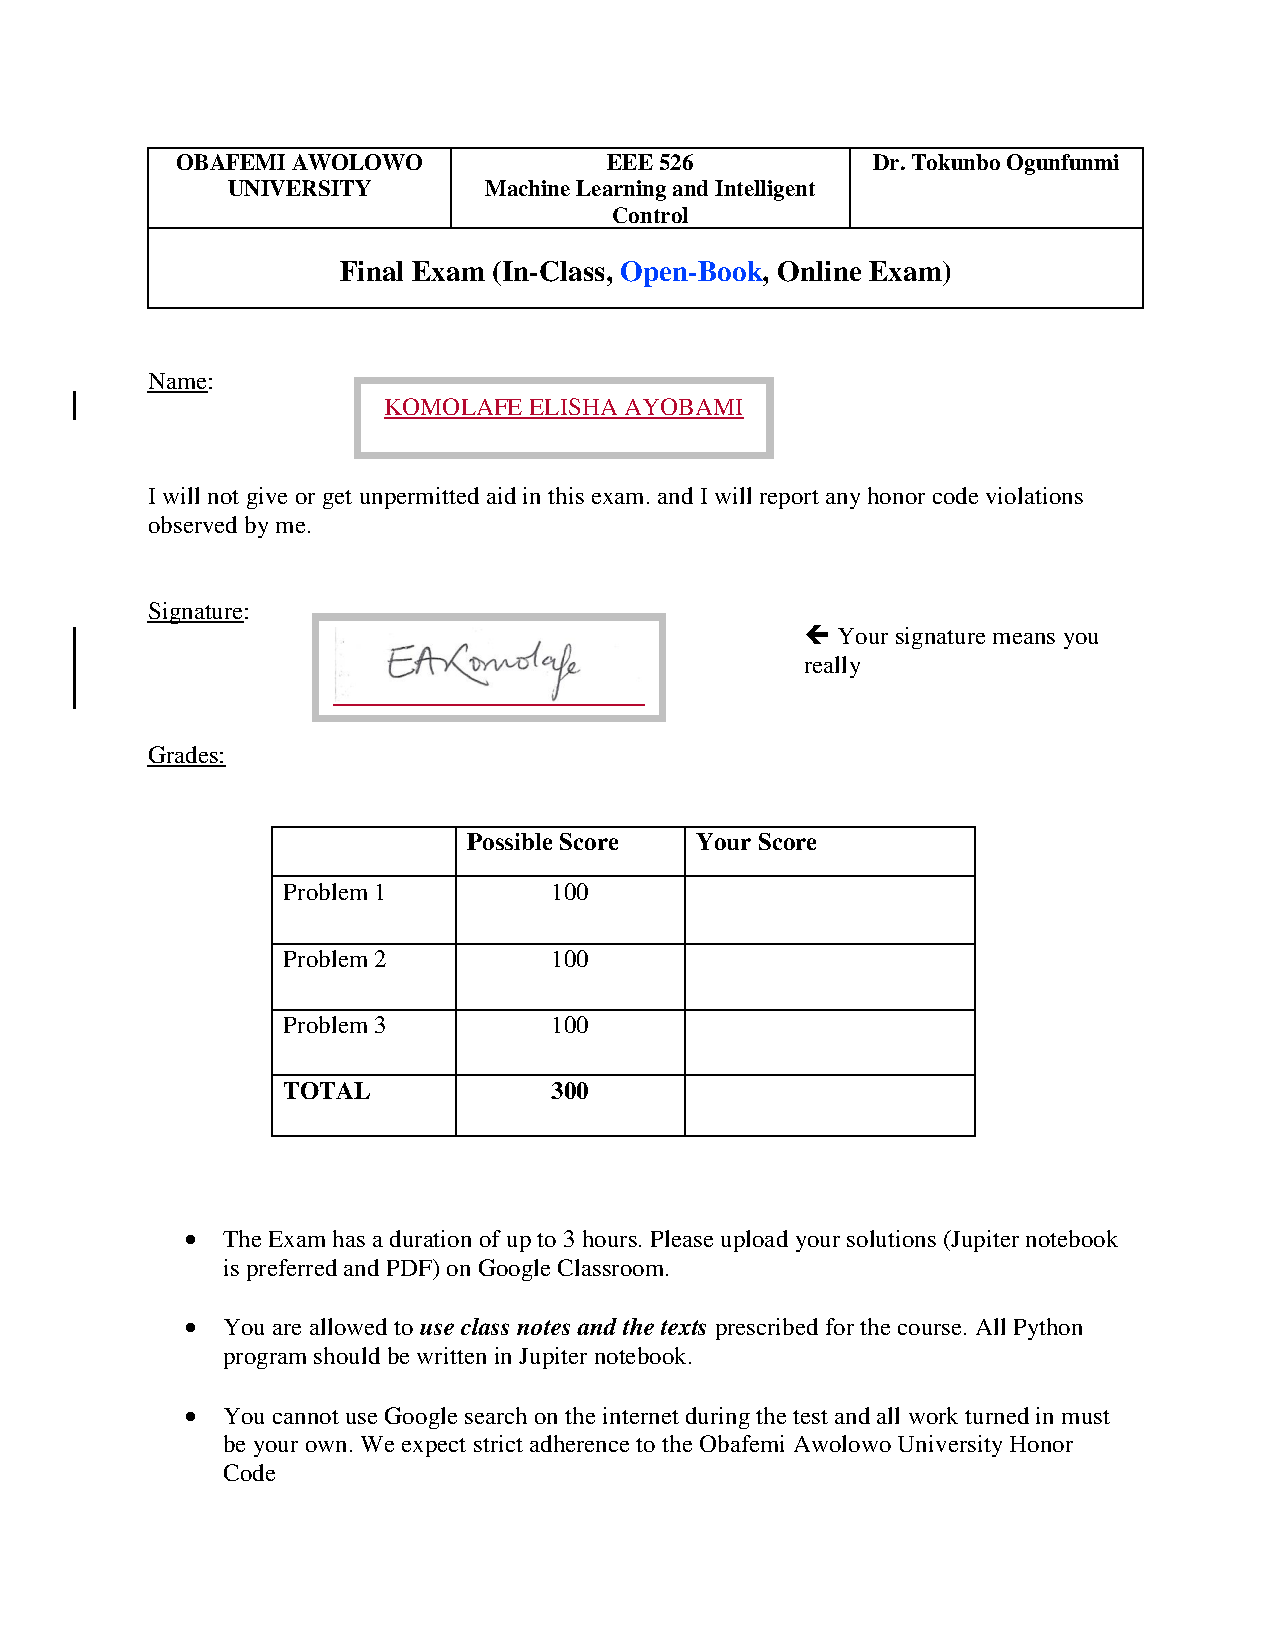
\includepdf[pages=1]{finalexam}

\newpage
\chapter{Investigating the space shuttle "Challenger" Accident using Logistic Regression}

\section{Fitting a Logistic model}
\subsection{data processing}
\subsection{what are the coefficients?}
the coefficients of the Logistic regression model for the classes 'No' and 'Yes', which tell us whether there is a probability of failure of not is, [-0.22950051]
\subsection{interpreting the coefficients}
the coefficients can be interpreted to the be weight that is applied to the temperature given to the model to calculate whether there will be a probability of failure with the o-rings.

\section{removing data for flight 18}
on removing the data from flight 18 the new coefficients for the model is [-0.32482337] which now shows there is a much higher reduction in the influence of temperature in the model.
\section{prediction for 31 degrees}
the probability of the o-ring failing at 31 degrees is Yes, which means the plane would crash if launched.
\chapter{Multiple Linear Regression}
\section{numerical and graphical summaries}
By using the matplotlib and seaborn libraries, histograms,boxplots and the pair plot of the data was generated.\\
The Data shows a high linear correlation among all the variables and each other
\section{significant predictors}
4 models which used each of the predictors as the dependent variable were created and based on the $R^{2}$ value the predictors can be listed based on how significant they are to the models.
\begin{itemize}
	\item EXAM 1,this is because the drop in the model without it shows a large decrease.
	\item EXAM 2
	\item EXAM 3
	\item FINAL 
\end{itemize}
\section{hypothesis testing}
assuming a hypothesis with the final exam model which says \emph{the final exam score of a student with average scores in the 3 exams is 50}
the t test values from the models shows the exam 1 is very significant thus dismissing the null hypothesis to accept the alternative which is with average scores a student will score higher in the final exam
\section{forcast prediction}
3 data for students were tested to generate the results of 83, 98 and 160 for the final scores
\chapter{Short Answer Questions}
\section{regression model choice}
\emph{In What cases would you use a Logistic Regression model instead of Linear Regression model?}\vspace{0.5cm}\\
The Main difference between a logistic and linear regression model is that is best used for classification problems while the other is used for regression problems.\\ The Linear Regression is a method that produces a straight line as the predicted relationship between the independent and dependent variables, this makes it very suitable in cases where continuous values are used, and are the predicted variables. \\
The Logistic Regression is a method that is best suited for classification problem where in there is distinct class for which the algorithm will be needed to choose between, e.g. classifying a set of input to either a pass or fail grade for a student.

\section{Explain why we need resampling methods?}
\subsection{3 Examples of re-sampling methods}
the Three types of re-sampling methods are:
\begin{itemize}
	\item Cross-Validation 
	\item Bootstrapping
	\item Pre-validation
\end{itemize}
\subsection{which re-sampling method would you use for an application and why?}
for the re-sampling methods listed above the applications I used them based on their operation are:
\vspace{0.5cm}\\
\textbf{Cross-validation}: this method involves splitting the training data into blocks for training, testing, and for some variants hold out.
the best application for the cross-validation resampling method is for a problem where the training data is not very large and the samples are large enough so as not to become computational intensive, and one where the training and test error might not be as low as they can be.
\vspace{0.5cm}\\
\textbf{Bootstrapping}: this method is similar to the cross-validation, but unlike the previous method where all the data available is used, not all are used here. this method involves splitting the data is chunks but instead of using all the data we replace some of it with repeated data. this method is used in problems that use time-series data such as EEG-data for stroke prediction where the data can be bootstrapped to generate more data.
\vspace{0.5cm}\\
\textbf{Pre-Validation}: unlike the previous methods which are used on data that corresponds to some output this method was designed to able to generate a fairer version of a independent used for comparison. this method is best suitable for Genetic studies and climate prediction where current data is biased with the result already and to be able to generate fair models for use.

\section{What is support Vector Machine(SVM)?}
A support Vector Machine (SVM) is a method used for solving classification problems in machine learning, it classifies a input based on which side of the hyperplane it is on. it is best used when there are only 2 classes to be classified with a linear decision boundary.

\section{Differentiate between K-Means Clustering and K-Nearest Neighbor (KNN)} 
Both methods are supervised learning methods where the output for the data is known. the difference between both methods ares:
\vspace{0.5cm}\\
\textbf{K-Means Clustering}: This method classifies data according to a cluster, which means each unique data can be identified by a cluster, the clusters are made by generating a `field' around all the data that have the same characteristics based on the variables used to classify them.
\vspace{0.5cm}\\
\textbf{K-Nearest Neighbor}: Unlike the method described above the KNN is not a method for clustering but a method for classification. 
\section{Differentiate between Linear Discriminant Analysis (LDA) and Quadratic Discriminant Analysis (QDA)}
both of the listed methods are  discriminant methods that are used when the classes to be divided are more than 2, but the difference between them is that while the LDA uses a linear spline to split the data, the QDA uses a higher order spline to split the data.
\end{document}